\subchapter{Creating a new virtual netdev}
{Objective: learn how to interact with net devices in the kernel, and use netlink}

\section{Goals}
 
 \begin{itemize}
 \item Create a very basic driver for a new Layer 2 network protocol
 \item Use \code{rtnl_link}
 \item Demonstrate stacked netdevice implementation
 \end{itemize}

\section{Bootlin LAN}

In the next few labs, we will be implementing our custom Tagging protocol. It is similar to 802.1Q VLAN, with the following differences:

\begin{itemize}
	\item Ethertype is ASCII "BL", or hex \code{0x424C}
	\item The BLAN id is encoded on 2 bytes, using the ascii representation of the tag's numerical value
	\item \textit{e.g.} BLAN id 12 has the tag "12" or hex \code{0x3132}
	\item Only one single BLAN can be added to a given trunk interface
\end{itemize}

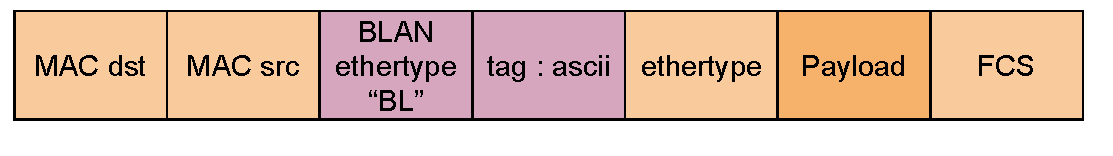
\includegraphics[width=0.7\textwidth]{labs/networking-netlink/ethernet_frame_blan.pdf}
 
\section{Compiling and loading our new driver}

For this lab, the code of the driver is located in \code{/home/$USER/networking-labs/target/blan}

This driver is out-of-tree, meaning that it is not compiled as part of the kernel, but as a separate kernel module.

To compile it, you need to use buildroot :
\begin{hostbashinput}
$ cd /home/$USER/networking-labs/buildroot
$ # Only re-compile the blan driver :
$ make bootlinlabs-blan-rebuild
$ # OR
$ # Only re-compile the blan driver and the full image
$ make bootlinlabs-blan-rebuild all
\end{hostbashinput}

After doing so, you need to re-flash your sdcard using \code{dd}.
 
You can now boot your Espressobin, and insert the module corresponding to our driver :
 
\begin{targetbashinput}
insmod blan.ko
\end{targetbashinput}
 
 You should see your Hello World message being printed out.
 
 \section{Adding a new rtnl\_link device type}
 
 Let's register our new link type to the \code{rtnl_link} family, by creating a
 new \code{rtnl_link_ops} object :
 
\begin{verbatim}
static struct rtnl_link_ops bootlinlan_link_ops = {
        .kind = "blan",
        .maxtype = IFLA_BLAN_MAX,
        .setup = bootlinlan_setup,
        .newlink = bootlinlan_newlink,
        .dellink = bootlinlan_dellink,
};
\end{verbatim}

 We will need some private data structure to be associated to our \kstruct{net_device}, that will store context to be used in all our callback functions.

 Create a new structure definition at the top of the file, for now empty :

\begin{verbatim}
struct bootlinlan_priv {
};
\end{verbatim}

To make sure that the \kstruct{net_device} associated to our new interface is allocated with enough
room in its \code{net_device.priv} field, we can pass the size of the private data in the \code{rtnl_link} info :

 \begin{verbatim}
 static struct rtnl_link_ops bootlinlan_link_ops = {
 ...
        .priv_size = sizeof(struct bootlinlan_priv),
 };
 \end{verbatim}
 
 We now need to populate the 3 callback functions that were mentionned : \code{bootlinlan_setup}, \code{bootlinlan_newlink} and \code{bootlinlan_dellink}.
 
 Take a look at the \kstruct{rtnl_link_ops} definition to know the signature of these functions.
 
 \code{bootlinlan_setup} will be called when the \code{rtnl_link} framework will allocate and initialize
 the \kstruct{net_device} that will be created when running the \code{ip link} command.
 
 There's 3 steps we need to take care of in the setup function :
 \begin{itemize}
 	\item Specify the \kstruct{net_device} information about the encapsulation (MTU, header size, etc). In our case, we can simply re-use the ones from a regular ethernet device by calling \kfunc{ether_setup}
 	\item As we are not dealing with a driver for a real device (yet), \code{rtnl_link} will allocate a \kstruct{net_device} for us. Therefore, we can make so that the networking stack also takes care of freeing the \kstruct{net_device} for us when we are done with it. This is done by setting \code{dev->needs_free_netdev} to \code{true}
	\item Finally, all \kstruct{net_device} objects need some NDOs (netdev ops) to be populated. Create a global variable of type \kstruct{net_device_ops}, and pass its address into \code{dev->netdev_ops}. Populate the only required member of the ops, \code{.ndo_start_xmit()}. You can make a dummy function that does nothing but \code{return NETDEV_TX_OK;}.
 \end{itemize}

 Let's now focus on \code{bootlinlan_newlink}. This is were we'll focus most of our efforts in this lab.

 This function takes as parameters :
 \begin{itemize}
	 \item \code{struct net *src_net} : The network namespace in which the new device is created
	 \item \code{struct net_device *dev} : The newly created \kstruct{net_device}, that we want to configure
	 \item \code{struct nlattr *tb[]} : A Netlink Attribute array containing attributes from the \href{https://elixir.bootlin.com/linux/v6.12.32/A/ident/IFLA_LINK}{RTNL Family}
	 \item \code{struct nlattr *data[]} : A Netlink Attribute array contaning attributes specific to our link type
	 \item \code{struct netlink_ext_ack *extack} : A Netlink Extended ACK object, for error reporting
 \end{itemize}

 In our case, the patched version of \code{iproute2} that is provided will :
 \begin{itemize}
	 \item Place the parent's interface index into \code{tb[IFLA_LINK]}, as a u32 value
		 \begin{itemize}
			\item \code{ip link add link }\textcolor{red}{\code{eth0}}\code{ name blan0 type blan id 10}
		 \end{itemize}
 \end{itemize}

 Check that the IFLA\_LINK value is provided (i.e that \code{tb[IFLA_LINK]} is not \code{NULL}). You can return \code{-EINVAL} if that's not the case.

You can retrieve the numerical values from attributes by using and \kfunc{nla_get_u32}.

The bootlinlan \code{id} is hardcoded in our drver, pick a value between 0 and 99, and store it in our local \code{bootlinlan_priv} struct for later use, make sure that you update the struct accordingly :

\begin{verbatim}
struct bootlinlan_priv {
        u16 id;
};
\end{verbatim}

A pointer to your private data structure is stored in \code{net_device.priv} :

\begin{verbatim}
struct bootlinlan_priv *priv = netdev_priv(dev);
\end{verbatim}

Then, you need to retrieve a pointer to the \textcolor{red}{parent} netdev. This will be used to configure our netdev.
To get a netdev from its index, you can call \kfunc{__dev_get_by_index}. Take a look at its documentation to know what are the expected parameters.

Now that you have a pointer tothe parent netdev, we can configure our device :

\begin{itemize}
	\item The \kstruct{device} that backs our netdev is the same as the parent's. We can use \code{SET_NETDEV_DEV(dev, &parent_dev->dev);} to set it.
	\item We want to inherit the same MAC address as the parent. Use \kfunc{eth_hw_addr_inherit} for that.
\end{itemize}

We can finally register our device ! We need to call either \kfunc{register_netdevice}, or \kfunc{register_netdev}. Only one of them will work in our case :)

Once your code compiles, reboot your board, insert the module, and try to add a new \code{blan} device :

\begin{targetbashinput}
ip link add link lan0 name blan10 type blan
\end{targetbashinput}

You should see your new device with :

\begin{targetbashinput}
ip link show
\end{targetbashinput}

You can now populate the \code{bootlinlan_dellink} function, that unregisters the device. In our case, we need to use
a special helper named \kfunc{unregister_netdevice_queue}, as we are currently holding the RTNL lock.

\section{Configuring the stacked net devices}

One final step is to notify the entire system that our \code{blan0} interface is stacked on \textcolor{red}{\code{lan0}}. To do this, add a call to \kfunc{netdev_upper_dev_link} after the registration of your netdev.

In the \code{bootlinlan_dellink}, the opposite is done by calling \kfunc{netdev_upper_dev_unlink}, however you'll notice that it takes as parameters both the \textcolor{red}{parent} device and our netdevice. So, let's add a \kstruct{net_device} field in the \code{bootlinlan_priv} data structure :

\begin{verbatim}
struct bootlinlan_priv {
        struct net_device *lowerdev;
        u16 id;
};
\end{verbatim}

